\documentclass[journal]{IEEEtran}

%%%%%%%%%%%%%%%%%%%%%%%%%%%%%%%%%%%%%%%%%%%%%%%%%%%%%%%%%%%%%%%%%%%%%%%%%%%%%%%%
%
% Package
%
%%%%%%%%%%%%%%%%%%%%%%%%%%%%%%%%%%%%%%%%%%%%%%%%%%%%%%%%%%%%%%%%%%%%%%%%%%%%%%%%
\usepackage{ifpdf}
\ifCLASSINFOpdf
  \usepackage[pdftex]{graphicx}
  % declare the path(s) where your graphic files are
  % \graphicspath{{../pdf/}{../jpeg/}}
  % and their extensions so you won't have to specify these with
  % every instance of \includegraphics
  \DeclareGraphicsExtensions{.pdf,.jpeg,.png}
\else
  % or other class option (dvipsone, dvipdf, if not using dvips). graphicx
  % will default to the driver specified in the system graphics.cfg if no
  % driver is specified.
  \usepackage[dvips]{graphicx}
  % declare the path(s) where your graphic files are
  % \graphicspath{{../eps/}}
  % and their extensions so you won't have to specify these with
  % every instance of \includegraphics
  \DeclareGraphicsExtensions{.eps}
\fi

\usepackage[utf8]{inputenc}
\usepackage[T1]{fontenc}
\usepackage[french, english]{babel}
\usepackage{cite}
\usepackage{caption}
\usepackage{amsmath,amsfonts,amssymb}
\usepackage{subcaption}
\usepackage{array}
\usepackage{color}
\usepackage{float}
\usepackage{multicol}
\usepackage[]{algorithm2e}
\usepackage{hyperref}
\usepackage{fancyhdr}
%
% correct bad hyphenation here
\hyphenation{op-tical net-works semi-conduc-tor}

\DeclareMathOperator*{\argmin}{arg\,min}
\DeclareMathOperator*{\argmax}{arg\,max}

\begin{document}
\pagestyle{plain}
\pagenumbering{arabic}


\appendix
\subsection{Algorithms}


\begin{algorithm}
 \KwData{$P_{i}$ series,\\ Grid policy $ (P^{MIN},\phi) $,\\ Desired number of coalitions $ N_{COAL} $,\\ size of starting cliques k}
 \KwResult{ $ CS = \{ S_{1},...,S_{N_{COAL}}\} $ }
 Compute $ G_{2}^{\epsilon^{\star}} $ \;
 Find the $ N_{COAL} $ cliques in $ G_{2}^{\epsilon^{\star}} $\;
 \While{$ \mathcal{U}(CS) $ is improving}{
 	\For{each clique}{
 		Find $ i^{\star} $ \;
 		\If{ $ \delta_{clique}(i^{\star}) \geq 0 $ }{
 			$ clique \leftarrow clique \cup \{i^{\star} \} $ \;
 			}
 		\If{ $ \exists j \in clique,\ s.t\ \delta_{clique}(j) < 0 $}{
 			$ clique \leftarrow clique - \{j \} $ \;
 			}
   		}
  	}
 \caption{Local greedy optimization algorithm}
 \label{alg:algo1}
\end{algorithm}

\begin{figure}[b]
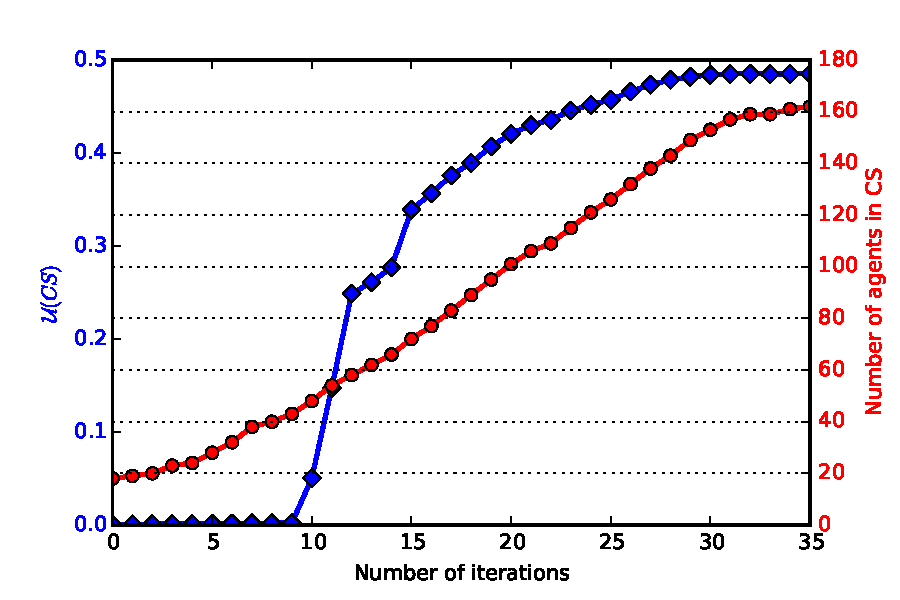
\includegraphics[scale=.5]{./figs/figure_7}
\caption{Evolution of the global utility $ \mathcal{U}(CS) $ (blue diamond curve, left axis) and the number of agents involved in the coalitions (red circle curve, right axis) during the greedy optimization of algorithm \ref{alg:algo1} }
\label{fig:search}
\end{figure}

Figure \ref{fig:search} displays the evolution of the global utility and the number of involved agents during the course of the greedy algorithm \ref{alg:algo1}. The transition from an invalid to a valid coalitions is clearly visible on the blue diamond curve and occurs between iteration 10 and 15. After this transition, coalition's utilities improve slowly up to a maximum point. 

\begin{algorithm}
 \KwData{Agent set $\mathcal{A}$,\\ Desired number of coalitions $ N_{COAL} $, \\ Maximum number of iterations $ Loop^{max} $}
 \KwResult{ $ CS = \{ S_{1},...,S_{N_{COAL}}\} $ }
 $ N^{loop} \leftarrow 0 $ \;
 $ CS^{\star} \leftarrow \emptyset $\;
 \While{$ N^{loop} < Loop^{max} $}{
 	$ CS \leftarrow SelectRandomCS( ) $\;
 	\If{ $ \mathcal{U}(CS) > \mathcal{U}(CS^{\star}) $ }{
 		$ CS^{\star } \leftarrow CS $\;
 		}
 	$ N^{loop} \leftarrow  N^{loop} + 1 $\;
  	}
  return $ CS^{\star} $
 \caption{Random algorithm}
 \label{alg:algo2}
\end{algorithm}

\begin{algorithm}
 \KwData{$P_{i}$ series,\\ Desired number of coalitions $ N_{COAL} $,\\ search step size $ \beta << 1 $}
 \KwResult{ $ CS = \{ S_{1},...,S_{N_{COAL}}\} $ }
 $ \epsilon \leftarrow 1 $ \;
 $ CS \leftarrow \emptyset $\;
 \While{$ |CS| < N_{COAL} $}{
 	Compute $ G_{1}^{\epsilon} $ \;
 	$ CS \leftarrow computeClusters( G_{1}^{\epsilon} ) $\;
 	\If{ $ |CS| = N_{COAL} $ }{
 		return CS\;
 		}
 	\Else{ 
 	$ \epsilon \leftarrow \epsilon - \beta $\;
 	}
  	}
 \caption{Correlated algorithm}
\label{alg:algo3}
\end{algorithm}


\subsection{Net production series}
\label{appendixB}

Data were collected from \cite{Infoclimat} (data for the United States at \cite{NCDC}). The variables used in the simulation are :

\begin{itemize}
\item Average wind speed (in $m.s^{-1}$)
\item Nebulosity (integer in $[0,8] $)
\item Temperature (in degree Celsius)
\end{itemize} 

\subsubsection{Wind power curve}
Power curves are functions that, for a given type of generator, map some input quantity to the output power produced. For wind-turbines and solar arrays these functions are well studied and approximations have been proposed \cite{Lydia2014} \cite{Piedallu2007, Piedallu2008}. For the wind turbines, the power curve can be specified by 4 values :

\begin{itemize}
\item Cut-in-speed : The wind speed at which the turbine first starts to rotate and generates power.
\item Rated-output-power : The maximum power that the turbine can generate.
\item Rated-output-speed : The wind speed at which the turbine attains its rated output power.
\item Cut-out-speed : The speed at which the turbine is turned off as not to damage the rotor.
\end{itemize}

The most interesting part is the increase of output power when the wind speed is in the cut-in-speed rated-output-speed range. Even if sometimes a simple linear model is used, the increase has been shown to be non linear and some more complex exponential fit can be found in the literature \cite{Lydia2014}.

\subsubsection{Solar power curve}
The input quantity desired for our power curve model for solar arrays is a radiance in $ W.m^{-2} $, which can be difficult to find in weather station available data. As we mainly collected nebulosity series, we used the Helios model described in \cite{Piedallu2007, Piedallu2008}. This model enabled us to compute perfect (clear blue sky situation) solar radiances at some specific locations on earth and at given timestamps. As nebulosity is a measure of the sky cloudiness, we can use the nebulosity series as degradation factors on the clear blue sky model (see \cite{Piedallu2007, Piedallu2008} for more details) :

\begin{equation}
\left\{ \begin{array}{lll}
			\Psi{real}(t) = \Psi_{perfect}(t) \eta(t) \\
			\eta(t) = 1-0.75 \left( \dfrac{N(t)}{8} \right)^{3.4}
\end{array} \right.
\end{equation}
where $ \Psi_{perfect}(t) $ and $ \Psi{real}(t) $ are respectively the clear blue sky and real radiances at time t, $ \eta(t) $ is the degradation factor at time t, and $ N(t) $ is the nebulosity index at time t. Once we have input data in the forms of radiances, we compute the production of a solar array with the following simplified power curve :

\begin{equation}
\mathcal{F}_{PV}(\Psi{real}(t)) =  S_{PV} \Psi{real}(t)  e_{PV}
\end{equation}
where $ S_{PV} $ is the surface of the array, and $ e_{PV} $ is its efficiency. The very simple form of this power curve is due to some simplifications in order not to overload the model. For instance, it does not take into account angles and orientations degradations. These could be incorporated if needed by changing the power curve in the simulations.

\subsubsection{Consumption}
Modeling electric consumption has already been widely tackled in the literature. Models can be basically divided into two main categories : Top-down and bottom-up approaches. Top-down techniques take aggregated consumption data as inputs and try to estimate individual consumption patterns while bottom-up methods use a fine modeling of users consumptions as to obtain realistic aggregated consumption curves. In this paper, we used a bottom-up model since the end user, or relatively small aggregations of end users, are in our interest. The main objective was to capture both daily patterns and seasonal variations of the consumptions. We assumed an additive model where the consumption of an agent is the sum of a seasonal heating term that depends on the outside temperature and an electronic consumption term that only depends on the hour of the day. By denoting $ \tau(t) $ the outside temperature at timestamp t, we can express the consumption $ P_{i}^{D}(t) $ of agent i at time t :

\begin{equation}
P_{i}^{D}(t) = \mathcal{F}_{i}^{heat}(\tau(t), t) + \mathcal{F}_{i}^{elec}(t)
\end{equation}
where $ \mathcal{F}_{i}^{heat}(\tau(t), t) $ is the power curve that maps the temperature to a heating consumption, and $ \mathcal{F}_{i}^{elec}(t) $ computes the consumption of agent i (other than heating) at a given hour of the day. In the simulation, all agents have a desired inside temperature $ T_{i} $, supposed to be a constant for simplification. By using thermodynamic laws $ \mathcal{F}_{i}^{heat}(\tau(t), t) $ can be approximated by :

\begin{equation}
\mathcal{F}_{i}^{heat}(\tau(t), t) = \dfrac{B_{i}}{R_{i}} \left[ T_{i} - \tau(t) \right]
\end{equation}
where $ B_{i} $ is the surface of thermal exchanges for agent i and $ R_{i} $ is their thermal resistance. We denote by $ \Omega_{i} $ the maximum consumption possible for agent i, which is basically the sum of all its appliances powers. We also denote by $ \omega_{i}(t) = \{ \omega_{i}(t_{0}),...,\omega_{i}(t_{24}) \} $ the vector of the average fraction of $ \Omega_{i} $ used for each hour. We can therefore write :

\begin{equation}
\mathcal{F}_{i}^{elec}(t) = \Omega_{i} ( \omega_{i}(t) + \epsilon )
\end{equation}
where $ \epsilon $ is a noise term. The vector $ \omega_{i}(t) $ enables us to easily differentiate agent consumption behaviors. Business or residential areas for instance can be easily distinguished with this kind of model.

\subsection{Resilience algorithm}
\label{appendix_resilience}
The following algorithm (see algorithm \ref{alg:algo4}) explains the process through which the resilience of a coalition structure is explored. For a given coalition structure, we consider random failures of physical components of the agents. This results in the agent being unable to support its coalition. Therefore, the agent is simply removed from the coalition, which impacts the coalition's production. Eventually, after some number of agent failures, some coalitions might not be sufficiently stable and productive to fulfill the market's constraints. In this case, the coalition fails, and is removed from the market.
\begin{algorithm}
	\KwData{$ CS = \left\{ S_1,S_2,...,S_k \right\} $ Coalition structure \;}
	
	$ pool = \cup_{k \in N_{COAL}} S_k $ \; 
	\While{ $ pool \neq \emptyset $}{
		Select randomly agent i from pool\;
		i fails $ \Rightarrow $ Remove i from its coalition : $ S_k \leftarrow S_k - \{i\} $ \;
		$ pool = pool - \{i\} $\;
		\If{ $ Pr \left[ P_{S_k} < P^{MIN} \right] > \phi $}{
			$S_k$ fails $ \Rightarrow $ Remove $S_k$ from the market
			} 
		}
	\caption{Random failures algorithm}
\label{alg:algo4}
\end{algorithm}


\bibliographystyle{IEEEtran}  
\bibliography{Article}
\end{document}